%!TEX root = ../report.tex
\section{Height plot}
\label{sec:height_plot}
All previous operations were implemented in a 2D plane.
While all previous operations were also most apt to implement in a 2D domain, it is a waste to not use an extra dimension which can convey extra information that might aid in visualizing a dataset.

To make use of this extra dimension we have implemented an option to view the scalar dataset as a height plot.
In a height plot, every point of the plane is warped along the surface normal proportionate to the scalar value at that point.
In the case of our simulation, we know that the surface is always pointed in the direction of the positive \texttt{z}-axis.
This property has eased implementation as all calls to \verb glVertex2f  can be replaced with a call to \verb glVertex3f  with the third parameter set to 0 if height plotting is not used, and the scalar value of the dataset otherwise.

Besides warping a dataset by the current dataset, which conveys enough interesting extra visual cues to the user as it is, it is also possible to warp a scalar dataset with the values of another scalar dataset. 
This effectively allows an user to view two scalar datasets at the same time by showing the color-mapped scalar values of one dataset with the height information of the other dataset. 

Of course, some controls must be provided to manipulate the view of the simulation in order to obtain the best visualization. 
We have accommodated this option by implementing three spinners which can alter the view angle around the \texttt{x}-, \texttt{y}- and \texttt{z}-axis between 0 and 360 degrees, providing vision on the simulation from every possible angle.
Moreover, we have implemented a simple spinner to implement zoom functionality. 
Using the spinner a zoom factor between 0.2 and 10 can be set, allowing for enough zoom possibility.
\begin{figure}[htb]
	  \centering
	  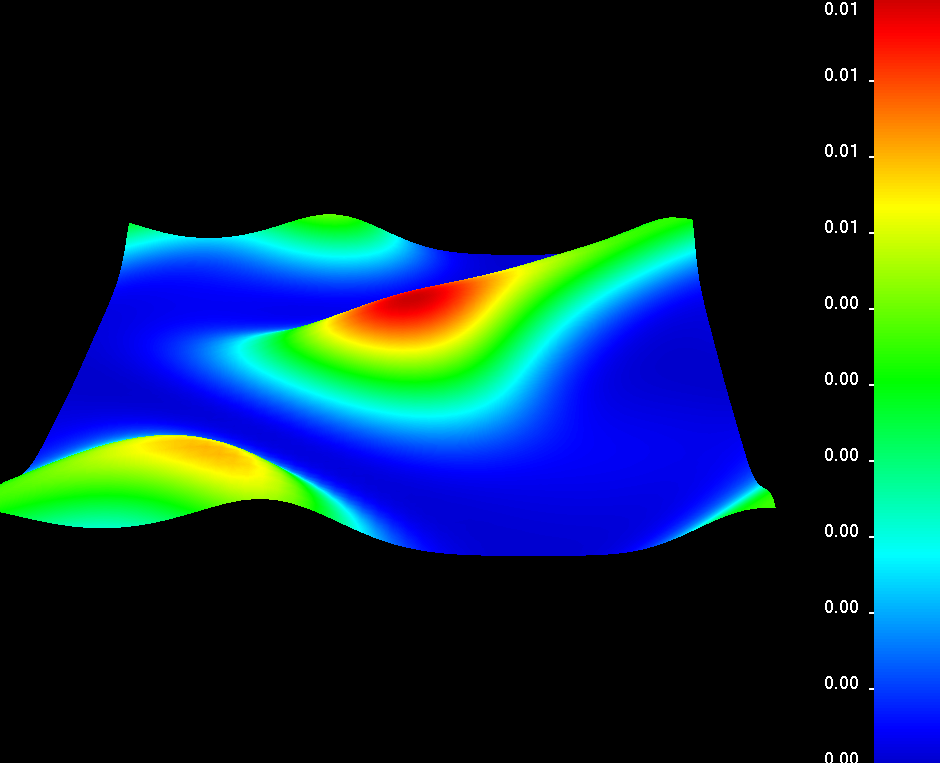
\includegraphics[width=\linewidth]{./content/pictures/heightplot.png}
	  \caption{The height plot of the fluid density dataset using the fluid density displacement set}
	  \label{fig:height_same}
\end{figure}
\begin{figure}[htb]
	  \centering
	  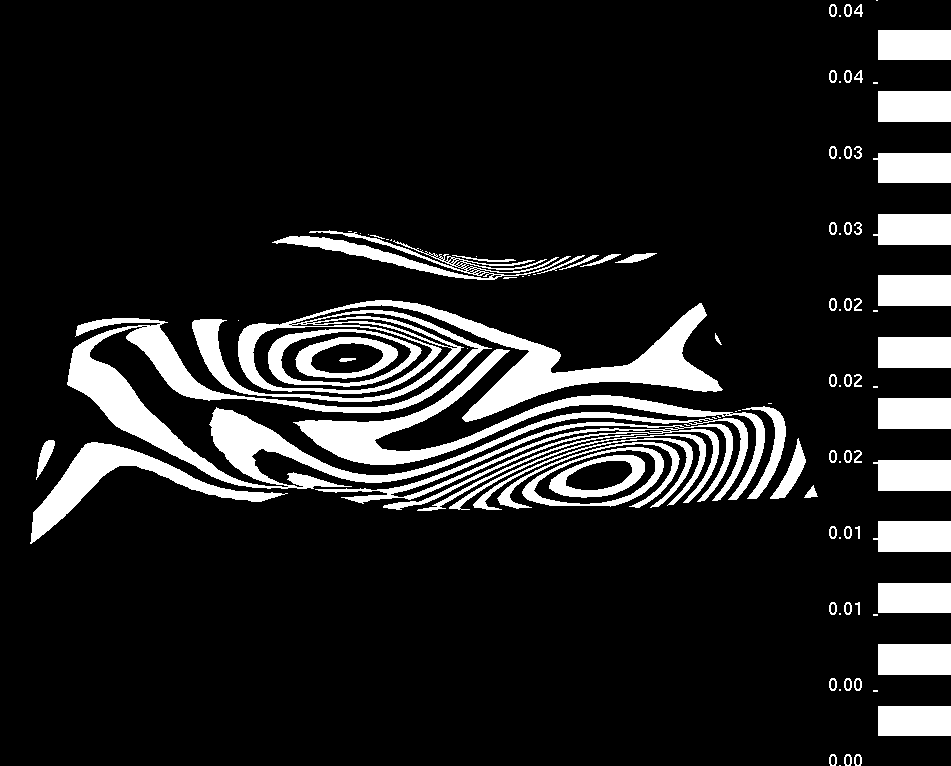
\includegraphics[width=\linewidth]{./content/pictures/heightplot_diff.png}
	  \caption{The height plot of the fluid density dataset using the the divergence of the velocity field as displacement set and zebra color map. Notice how densely banded areas occur at highly curved areas.}
	  \label{fig:height_diff}
\end{figure}

Certain combinations of datasets, displacement datasets and color mapping may provide a rich and detailed description of the data, as figure~\ref{fig:height_diff} illustrates.
The \(\rho\) dataset is visualized using a zebra color map, but displaced using the divergence of the velocity field, \(\nabla \mathbf{v}\).

% In order to implement a height plot, a conversion from 2D to 3D is needed.
% This can be done by converting the \texttt{glVertex2f(x, y)} to \texttt{glVertex3f(x,y,z)} in the function \texttt{draw\_smoke}.
% \texttt{x, y} are already known, \texttt{z} will become the value of a selected dataset, which can differ from the dataset that is used for the colormap.
% When heights are not plotted, \texttt{z} can be simply set to 0, this creates the already existing 2D plot.

% When converting to 3D, a problem arises that you need to specify the view point and view volume.
% In other words, the specification of the camera and bounding boxes need to be set.
% This problem can be fixed by using \texttt{gluLookAt, gluPerspective, glRotatef} and \texttt{glTranslatef}.

% Rotation of the simulation grid is done by first translating to the center of the grid and from that point the rotations are performed so that the center stays does not move.

% The color legend is drawn separately in 2D, so it will have a fixed position on the screen.
\clearpage